% ::setlocal makeprg=cd\ latex\ &&\ pdflatex\ -interaction=batchmode\ main.tex\ &&\ xdg-open\ main.pdf\ &&\ exit

\textit{The content of this chapter is mostly based on
\fullcite{hartle2021gravity} and \fullcite[ch. 12]{shapiro2008black}.}


\section{Introduction}

\subsection{Why the \Sh Geometry}

Newtonian mechanics is built upon the concept of absolute time and space.
Once the concept of \textit{inertial frame} is well-defined, physics can be
done on a space described by Euclidean geometry.
Free particles (particles on which no forces are acting) move in a straight
line, which is the shortest distance between two points in a three-dimensional
space, measured as:

\begin{equation}
    \Delta s^2 = \Delta x^2 + \Delta y^2 + \Delta z^2 \, .
    \label{cap1:eq:euclide}
\end{equation}

On the other hand, time is \textit{just} seen as a parameter, common to every 
inertial frame, that can be used to determine the particle velocity and
acceleration.

With the appearance of Maxwell's Equations it became clear that what they 
predicted (the speed of light being constant in every inertial frame) was in
contrast with the description of our space given by Newtonian Mechanics, where
the speed of anything changes with respect to the inertial frame chosen.
Between Maxwell's Equations and Newtonian mechanics Einstein chose to modify 
the latter and wrote his two postulates for the theory of Special Relativity:

\begin{itemize}
    \item The laws of physics are invariant (identical) in all inertial frames
        of reference;
    \item The speed of light in vacuum,
        $c = \num{299792458} \unit[per-mode = symbol]{\meter\per\second}$,
        is the same for all observers, regardless of the motion of light source
        or observer.
\end{itemize}

The postulates may or may not be intuitive, but simple observations based on
them bring us to abandon the idea of absolute space and time and to introduce
the concept of \textit{spacetime}, together with a new way of measuring
distances

\begin{equation}
    \Delta s^2 = - c^2 \Delta t^2 + \Delta x^2 + \Delta y^2 + \Delta z^2 \, .
    \label{cap1:eq:Minkowski}
\end{equation}

In special relativity distances measured this way are the same for every
observer in every inertial frame possible.

The appearance of time in a formula that is supposed to give us the distance
between two objects is surely destabilizing at first, but geometry teaches us
that fixing the way we calculate $\Delta s^2$, more properly referred to as the
\textit{line element} $\mathrm{d}s^2$, is enough to describe the geometry of
the space that we are using.
Since eq. \ref{cap1:eq:Minkowski} is different from eq. \ref{cap1:eq:euclide},
in
particular there is a minus sign in front of $\Delta t^2$, we moved away from
the familiar three-dimensional Euclidean geometry and are now in
four-dimensional spacetime, usually referred to as \textit{flat spacetime} or
\textit{Minkowski space}.

This new geometry allowed for a reformulation of Maxwell's Equations and
brought (and explained) phenomena like time dilation, length contraction and the
relativity of simultaneity.
The last one in particular, the concept that the simultaneity of two events
depends on the frame of reference, poses a threat to the \textit{force} of
gravity.
Up until this point gravity was defined as the instantaneous force $F_{12}$
acting on a mass $m_1$ at time $t$ due to a second mass $m_2$:

\begin{equation}
    F_{12} = G \frac{m_1 m_2}{|r_1(t) - r_2(t)|^2}
    \label{cap1:eq:force_of_gravity}
\end{equation}

The adjective \textit{instantaneous} in a theory where nothing can travel
faster than the speed of light should already raise some concern.
But looking at $r_1(t)$ and $r_2(t)$ in eq. \ref{cap1:eq:force_of_gravity},
that are
supposed to indicate the positions of the masses in the same instant of time,
makes it even clearer that the force $F_{12}$ can't be the same in all
frames of reference.

Solving this issue gave birth to the theory of general relativity, where a mass
is not a source of gravitational force anymore, but is responsible for
bending the four-dimensional spacetime itself.
This implies that when we observe a particle deviating its trajectory from a
straight line in the presence of a massive object, it is not because of a force
acting on it.
In fact, we can consider the particle free and moving from point A to point B
along the shortest path, it is just that in the curved surface bent by the mass
the shortest path is not a straight line.

While this concept may not enhance our intuitive understanding, the
implications and the mathematical formalism required to articulate the theory
are even more challenging.
If the presence of mass distorts the space we work in, changing the line
element $\mathrm{d}s^2$ is therefore necessary.
The details of the theories, particularly the Einstein field equations, that
describe this distortion and allow us to evaluate the new $\mathrm{d}s$ from a
give distribution of mass are beyond the scope of this thesis.
Our focus will be on evaluating the observable effects, given the line
element.

More specifically we will study one of the simplest curved spacetime that
general relativity has to offer: the geometry of empty space outside a
spherically symmetric source of curvature, for example, a spherical
star.
It is one of the simplest because of the many symmetries that presents and,
luckily, is also one of the most useful.

The line element of what is more commonly know as the \Sh geometry is

\begin{equation*}
    \mathrm{d}s^2 = - \left(1 - \frac{2 G M}{c^2 r} \right) (c \mathrm{d}t)^2
    + \left(1 - \frac{2 G M}{c^2 r} \right)^{-1} \mathrm{d}r^2
    + r^2 (\mathrm{d}\theta^2 + \sin^2 \theta \mathrm{d}\phi^2)
\end{equation*}

expressed in spherical coordinates centered in the mass responsible for bending
the space.

\newpage


\subsection{Notation and Formalism}
\label{cap1:ssec:notation}

In the \textit{flat spacetime} we can introduce a coordinate basis for
four-vectors
\begin{equation}
    \mathbf{e_t} = (1,0,0,0), \quad
    \mathbf{e_y} = (0,1,0,0), \quad
    \mathbf{e_y} = (0,0,1,0), \quad
    \mathbf{e_z} = (0,0,0,1).
    \label{cap1:eq:coord_base}
\end{equation}
The set 
$\{ \mathbf{e_t}, \mathbf{e_x}, \mathbf{e_y}, \mathbf{e_z} \}$, is often
referred to as $\{ \mathbf{e_0}, \mathbf{e_1}, \mathbf{e_2}, \mathbf{e_3} \}$.
Any four-vector $\textbf{a}$ can then be written as

\begin{equation}
    \textbf{a}
    = a^t \mathbf{e_t} + a^x \mathbf{e_x} + a^y \mathbf{e_y} + a^z \mathbf{e_z}
    = a^0 \mathbf{e_0} + a^1 \mathbf{e_1} + a^2 \mathbf{e_2} + a^3 \mathbf{e_3}
    \label{cap1:eq:a}
\end{equation}

where $(a_t,~a_x,~a_y,~a_z)$, or equivalently $(a_0,~a_1,~a_2,~a_3)$, are the
components of the four-vector.
Both notations will be used.

Another useful convention is to use Roman letters (usually $i$ or $j$) to refer
to indices 1, 2, 3 and Greek letters (usually $\mu$ or $\nu$) to refer to
indices 0, 1, 2, 3.
Using Einstein notation the expression in eq. \ref{cap1:eq:a}, can be rewritten
simply as $\textbf{a} = a^\mu \mathbf {e_\mu}$.
Other useful ways to specify the components of $\textbf{a}$ are

\begin{equation*}
    a^\mu = (a^t, a^x, a^y, a^z) \quad a^\mu = (a^t, a^i) \quad a^\mu
    = (a^t, \vec a)
\end{equation*}

where $\vec a = a^i e_i$ is the tree-dimensional vector $(a_x, a_y, a_z)$.

The length of the four-vector $\mathbf{a}$ must match the definition given with
the $\Delta s^2$ in \ref{cap1:eq:Minkowski}, it is useful to define the
\textit{metric} $\eta_{\nu \mu}$ so that

\begin{equation}
    \eta_{\nu \mu} = 
    \begin{array}{cc}
        \begin{pNiceMatrix}[first-row,first-col][columns-width = auto]
              & t & x & y & z \\
            t~~ & -1 & 0 & 0 & 0 \\  
            x~~ & 0 & 1 & 0 & 0 \\ 
            y~~ & 0 & 0 & 1 & 0 \\
            z~~ & 0 & 0 & 0 & 1 \\
        \end{pNiceMatrix} &
    \end{array}
    \quad \implies \quad
    \mathrm{d}s^2 = \eta_{\nu \mu} \mathrm{d}x^\nu \mathrm{d}x^\mu
\end{equation}

where a double sum is implied, and we rightfully notice that the minus sign has
appeared again under the $t$ component.
Now we can compactly write

\begin{equation}
    \mathbf{a} \cdot \mathbf{a} = \eta_{\mu \nu} \, a^\mu \, a^\nu
    = - (a^t)^2 + (a^x)^2 + (a^y)^2 + (a^z)^2
\end{equation}

Without any claim of rigorously demonstrating it, we can say that since this
scalar product is built from the line element $\mathrm{d}s^2$, it is the same
in every inertial frame one might choose. Quantities that have these properties
are \textit{invariant}.

When working in the \Sh geometry it is useful to adopt the \Sh coordinates,
spherical coordinates centered at the center of the mass $M$, and use
geometrized units, where $G = c = 1$ (Appendix \ref{ap:geometrized_units}).
The line element and the metric can be rewritten as

\begin{equation*}
    \mathrm{d}s^2 = - \left(1 - \frac{2 M}{r} \right) (\mathrm{d}t)^2
    + \left(1 - \frac{2 M}{r} \right)^{-1} \mathrm{d}r^2
    + r^2 (\mathrm{d}\theta^2 + \sin^2 \theta \mathrm{d}\phi^2)
\end{equation*}

\begin{equation}
    g_{\nu \mu} = 
    \begin{array}{cc}
        \begin{pNiceMatrix}[first-row,first-col][columns-width = auto]
              & t & r & \theta & \phi \\
            t~~ & - (1 - 2 M /r) & 0 & 0 & 0 \\  
            r~~ & 0 & (1 - 2 M /r)^{-1} & 0 & 0 \\ 
            \theta~~ & 0 & 0 & r^2 & 0 \\
            \phi~~ & 0 & 0 & 0 & r^2 \sin^2 \theta \\
        \end{pNiceMatrix} &
    \end{array}
    .
    \label{cap1:eq:Sh_g}
\end{equation}

It's worth pointing out that, given \ref{cap1:eq:Sh_ds}, the coordinate basis
introduced in \ref{cap1:eq:coord_base} is not normalized in this geometry, for
example:

\begin{equation}
    \mathbf{e_t \cdot e_t} = g_{\nu \mu} e_t^\mu e_t^\nu = g_{00}
    = - (1 - 2 M /r)
\end{equation}

If we want an orthonormal tetrad we can define

\begin{subequations}
\begin{align}
    \mathbf{\hat e_t} &= \left(1 - \frac{2M}{r}\right)^{-1/2} \mathbf{e_t}
    \quad &&\implies \quad
    \mathbf{\hat e_t \cdot \hat e_t} = g_{\nu \mu} \hat e_t^\mu \hat e_t^\nu
    = g_{00} \left(1 - \frac{2M}{r}\right)^{-1} = - 1
    \label{cap1:eq:local_ON_base_t}\\
    %
    \mathbf{\hat e_r} &= \left(1 - \frac{2M}{r}\right)^{1/2} \mathbf{e_r}
    \quad &&\implies \quad
    \mathbf{\hat e_r \cdot \hat e_r} = g_{\nu \mu} \hat e_r^\mu \hat e_r^\nu
    = g_{00} \left(1 - \frac{2M}{r}\right) = 1 \\
    %
    \mathbf{\hat e_\theta} &= \frac{1}{r} \mathbf{e_t}
    \quad &&\implies \quad
    \mathbf{\hat e_\theta \cdot \hat e_\theta} = 1 \\
    %
    \mathbf{\hat e_\phi} &= \frac{1}{r \sin \theta} \mathbf{e_t}
    \quad &&\implies \quad
    \mathbf{\hat e_\phi \cdot \hat e_\phi} = 1
\end{align}
    \label{cap1:eq:local_ON_base}
\end{subequations}

\newpage


\section{Proprieties of the Metric}

Let's first analyze the \Sh metric in more detail:

\begin{equation}
    \mathrm{d}s^2 = - \left(1 - \frac{2 M}{r} \right) (\mathrm{d}t)^2
    + \left(1 - \frac{2 M}{r} \right)^{-1} \mathrm{d}r^2
    + r^2 (\mathrm{d}\theta^2 + \sin^2 \theta \mathrm{d}\phi^2)
    \label{cap1:eq:Sh_ds}
\end{equation}

There are two singularities in $r = 0$ and $r = 2M$.
The first one is intrinsic to the spherical coordinate system and, since the
metric is only valid in the space outside the start, doesn't concern us.
The second occur at what is defined as the \textit{\Sh radius} $r_s = 2M$.
Every non-black hole object has a radius larger than its \Sh radius.
The nature and significance of this will become clearer in the subsequent
sections.

On the other hand, if we take the limit as $r$ approaches infinity, we notice
that the
metric becomes asymptotically flat, approaching the metric of \Mi space.

Finally, $\mathrm{d}s^2$ is independent of the coordinates $t$ and $\phi$.
This is expected, as the mass responsible for curving the spacetime is static
and spherically symmetric.
The metric’s independence from time and rotation implies the existence of two
easy \textit{killing vectors}:

\begin{equation}
    \xi = (1, 0, 0, 0) \quad \text{and} \quad \eta = (0, 0, 0, 1) \, .
    \label{cap1:eq:xi_eta}
\end{equation}

A \textit{killing vector} is a direction in the four-dimensional spacetime
along which we can freely move without changing the metric.
It is a general way to describe a symmetry of the metric.
Since symmetries correspond to conserved quantities they will be a key point in
studying the trajectories of free particles, the \textit{geodesics}.

We start by considering the four-momentum $\mathbf{p}$ of a particle of mass
$m$, defined as

\begin{equation}
    p^\mu := m u^\mu = m \dv{x^\mu}{\tau}
\end{equation}

where $u$ is the four-velocity of the particle, $x$ its position and $\tau$ the
proper time.
Therefore, the quantities

\begin{align*}
    E &= - \mathbf{\xi \cdot p} =
    - g_{00} \, p^0 = m \left( 1 - \frac{2M}{r} \right) \dv{x^t}{\tau} \\
    L &= \mathbf{\eta \cdot p} =
    g_{33} \, p^\phi = m r^2 \sin^2 \theta \dv{x^\phi}{\tau}
\end{align*}

will be conserved along the geodesic.
We already named them $E$ and $L$ as they are respectively the energy and the
angular momentum at large $r$ and low velocities.
To simplify the expressions used in the discussion will use renormalized
quantities

\begin{subequations}
    \begin{align}
        e &= \frac{E}{m} = \left( 1 - \frac{2M}{r} \right) \dv{x^t}{\tau}
        \label{cap1:eq:conserved_e} \\
        \ell &= \frac{L}{m} = r^2 \sin^2 \theta \dv{x^\phi}{\tau} \, .
        \label{cap1:eq:conserved_l}
    \end{align}
\end{subequations}

$e$ and $\ell$ are respectively the conserved energy and angular momentum per
unit
rest mass.

In the next sections the normalization of the four-velocity $\mathbf u$ will be
really useful too

\begin{subequations}
    \begin{align}
        &\mathbf{u \cdot u} = g_{\nu \mu} u^\nu u^\mu = -1 
        &&\text{for } m \neq 0 \label{cap1:eq:u_normalization_mass} \\
        &\mathbf{u \cdot u} = g_{\nu \mu} u^\nu u^\mu = 0 
        &&\text{for } m = 0 \label{cap1:eq:u_normalization_light} \, .
    \end{align}
    \label{cap1:eq:u_normalization}
\end{subequations}

It's not a property of the metric, but it's valid for every $g_{\nu \mu}$.
Equations \ref{cap1:eq:u_normalization} can be derived like this

\begin{align*}
    \mathrm{d}s^2 &= g_{\nu \mu} \mathrm{d}x^\nu \mathrm{d}x^\mu \\
    \dv{s^2}{\tau^2} &= g_{\nu \mu} \dv{x^\nu}{\tau} \dv{x^\mu}{\tau} \, .
\end{align*}

From here we use $\mathrm{d}s^2 = 0$ for a light ray, or the definition of
proper time $\mathrm{d}\tau^2 = - \mathrm{d}s^2$ for a massive particle.


\section{Gravitational Redshift}

Let's consider a static observer in $r$.
When the observer measures the energy of a photon, that corresponds to the $t$
component of $\mathbf{p}$, they do that using their local orthonormal tetrad
that we described in \ref{cap1:eq:local_ON_base}.

Referring to $p^{\hat t}$ as the value measured in the orthonormal tetrad
$\{\hat e_t, \hat e_r, \hat e_\theta, \hat e_\phi \}$ and
$p^t$ as the value measured with the coordinate basis
$\{e_{t}, e_{r}, e_{\theta}, e_{\phi} \}$, the energy measured in $r$ will be

\begin{equation*}
    E(r) = p^{\hat t} = \mathbf{p \cdot \hat e_t}
    = \mathbf{p \cdot e_t} \left(1 - \frac{2M}{r} \right)^{-1/2}
    = \mathbf{p \cdot \xi} \left(1 - \frac{2M}{r} \right)^{-1/2}
\end{equation*}
\begin{equation}
    \left(1 - \frac{2M}{r} \right)^{1/2} E(r) = \mathbf{p \cdot \xi}
    = \text{const} \, .
    \label{cap1:eq:photon_energy1}
\end{equation}

Where we used the expression for $\hat e_t$ from eq.
\ref{cap1:eq:local_ON_base_t}
and notice that $\mathbf{e_t} = \xi$ from eq. \ref{cap1:eq:coord_base} and eq.
\ref{cap1:eq:xi_eta}. 
Solving for the constant $\mathbf{p} \cdot \xi$ we find the expression in
\ref{cap1:eq:photon_energy1}. The relationship between the energy of a photon
measured at $r'$ and the one measured at $r$ from two static observers using
their own tetrad is

\begin{equation*}
    \left(1 - \frac{2M}{r'} \right)^{1/2} E(r')
    = \left(1 - \frac{2M}{r} \right)^{1/2} E(r)
\end{equation*}

Taking the limit as $r'$ approaches infinity and using $E = \hbar \omega$ for
the energy of the photon

\begin{equation}
    \omega_\infty = \omega_* \left(1 - \frac{2M}{r} \right)^{1/2} \, .
    \label{cap1:eq:redshift}
\end{equation}

Here, $\omega_\infty$ is the frequency measured by a distant observer at
$r \gg r_s$, while $w_*$ denotes the frequency measured at a specific distance
$r$.
Photons observed at a certain distance from a star exhibit a lower frequency
compared to the one they have at the point of emission.


\section{Particle Orbits}
\label{cap1:sec:particle_orbits}

\begin{minipage}{0.4 \textwidth}

% 3D AXIS with spherical coordinates
\tdplotsetmaincoords{60}{110}
\begin{tikzpicture}[scale=2,tdplot_main_coords]
  
    % Red vector coordinates
    \def\rvec{1.15}
    \def\thetavec{90}
    \def\phivec{70}
    
    % AXES
    \coordinate (O) at (0,0,0);
    \draw[thick,->] (0,0,0) -- (2,0,0) node[right=1]{$x$};
    \draw[thick,->] (0,0,0) -- (0,2,0) node[above=1]{$y$};
    \draw[thick,->] (0,0,0) -- (0,0,2) node[left=1]{$z$};
    
    % VECTORS
    \tdplotsetcoord{P}{\rvec}{\thetavec}{\phivec}
    \draw[thick,red] (O)  -- (P) node[below right]
        {$(r, \theta = \frac{\pi}{2}, \phi)$};
    %\draw[dashed]   (O)  -- (Pxy);
    \draw[dashed]   (P)  -- (Pxy);
    
    % ARCS
    \tdplotdrawarc[thick,->]{(O)}{0.4}{0}{\phivec} {anchor=north}{$\phi$}
    \tdplotsetthetaplanecoords{\phivec}
    \tdplotdrawarc[thick,->,tdplot_rotated_coords]{(0,0,0)}{0.5}{0}{\thetavec}
        {anchor=south west}{\hspace{-1mm}$\theta$}

    % Particle trajectory in XY plane
    \draw[thick,green,domain=-1.5:1.8,samples=100,variable=\t] 
        plot (\t, {1.5 - 1/(\t + 2)}, 0);
    % Dashed at the beginning
    \draw[thick,green,dashed,domain=1.8:2.3,samples=100,variable=\t] 
        plot (\t, {1.5 - 1/(\t + 2)}, 0);
    % Dashed at the end
    \draw[thick,green,dashed,domain=-1.55:-1.52,samples=100,variable=\t] 
        plot (\t, {1.5 - 1/(\t + 2)}, 0);

    % Center Point
    \shade[inner color=white, outer color=blue!60!black] (0,0,0) circle (3pt);

\end{tikzpicture}
\captionof{figure}{Visual representation of the spherical coordinates used.
The green line represents a possible trajectory on the $xy$ plane. \\}
\label{cap1:fig:spherical_coordinates}
\end{minipage}
\hspace{0.02 \textwidth}
\begin{minipage}{0.57 \textwidth}
    To further analyze the \Sh geometry, we will now explore the behavior of a
    test particle within it.
    A \textit{test particle} refers to an object with mass so small that its
    influence on the surrounding spacetime is negligible, allowing us to
    analyze its motion without altering the geometry of the spacetime itself.

    As already established from eq. \ref{cap1:eq:conserved_l} the angular
    momentum is conserved during the motion of a particle in this geometry.
    This implies that the particle's orbit must lie within a plane.
    Without loosing generality we can imagine the particle path to stay in the
    $xy$ plane, fixing $\theta = \pi / 2$ and, consequently,
    \begin{equation*}
        u^\theta = \dv{\theta}{\tau} = 0 
    \end{equation*}
    \begin{equation*}
        \ell = r^2 \sin^2 \theta \dv{\phi}{\tau} = r^2 \dv{\phi}{\tau}
    \end{equation*}

    Refer to Figure \ref{cap1:fig:spherical_coordinates} for a visual
    representation.
\end{minipage}
\hspace{0.02 \textwidth}

The four-velocity of our test particle can then be written as
\begin{equation*}
    u^\mu
    = \left(\dv{x^t}{\tau}, \dv{x^r}{\tau}, \dv{x^\theta}{\tau},
    \dv{x^\phi}{\tau} \right)
    = \left(\dv{t}{\tau}, \dv{r}{\tau}, 0, \frac{\ell}{r^2} \right) \, .
\end{equation*}

Where we simplified the notation using $t = x^t$ and $r = x^r$.
Thanks to the normalization of $\mathbf u$ (eq.
\ref{cap1:eq:u_normalization_mass}) and using $\theta = \pi / 2$ again, we can
write

\begin{equation*}
    - 1 = g_{\nu \mu} u^\nu u^\mu =
    - \left(1 - \frac{2M}{r} \right) \left(\dv{t}{\tau} \right)^2
    + \left(1 - \frac{2M}{r} \right)^{- 1} \left(\dv{r}{\tau} \right)^2
    + \frac{\ell^2}{r^2}
\end{equation*}

By using the conserved energy per unit rest mass found in
\ref{cap1:eq:conserved_e} to eliminate the dependence from $t$ and rearranging
the expression, we have

\begin{equation}
    e^2 = \left(\dv{r}{\tau}\right)^2 + \left(1 + \frac{\ell^2}{r^2}\right)
    \left(1 - \frac{2M}{r} \right) \, .
   \label{cap1:eq:found_e}
\end{equation}

To compare eq. \ref{cap1:eq:found_e} with the Newtonian case we can expand
the multiplication, subtract 1 from both sides and divide by a factor of 2:

\begin{equation}
    \mathcal E = \frac{e^2 - 1}{2} = \frac{1}{2} \left(\dv{r}{\tau}\right)^2
    + \frac{\ell^2}{2 r^2} - \frac{M}{r} - \frac{M \ell^2}{r^3} \, .
    \label{cap1:eq:found_epsilon}
\end{equation}

By defining this dimensionless constant $\mathcal E$, we can now see the
derivative of $r$ as the kinetic energy (per unit rest mass) and the other
terms as an effective potential acting on the particle, defined as

\begin{equation}
    V_{\rm eff}(r)
    = \frac{\ell^2}{2 r^2} - \frac{M}{r} - \frac{M \ell^2}{r^3} \, .
    \label{cap1:eq:V_eff}
\end{equation}

To better understand eq. \ref{cap1:eq:V_eff}, we can express it in
$\mathcal{LMT}$ units, substituting $\ell \rightarrow \ell / c$ and 
$ M \rightarrow G M / c^2$

\begin{equation*}
    V_{\rm eff}(r)
    = \frac{1}{c^2} \left( \frac{\ell^2}{2 r^2} - \frac{G M}{r}
    - \frac{G M \ell^2}{c^2 r^3} \right)
\end{equation*}
The first two terms are identical to the Newtonian potential for a particle
with angular momentum (per mass) $\ell$, orbiting around an object of mass $M$.
The third one is new, ignorable for $GM\ell^2 \ll c^2 r^3$, and it is
proportional
to $r^{-3}$.

Figure \ref{cap1:fig:V_effvsVN} shows the effect of the $r^{-3}$ term: the
infinite centrifugal barrier of the Newtonian potential disappears in
$V_{\rm eff}$ and a particle with enough energy can fall to the center of the
massive object.

\begin{figure}[h]
\begin{minipage}{0.49 \textwidth}
    \centering
    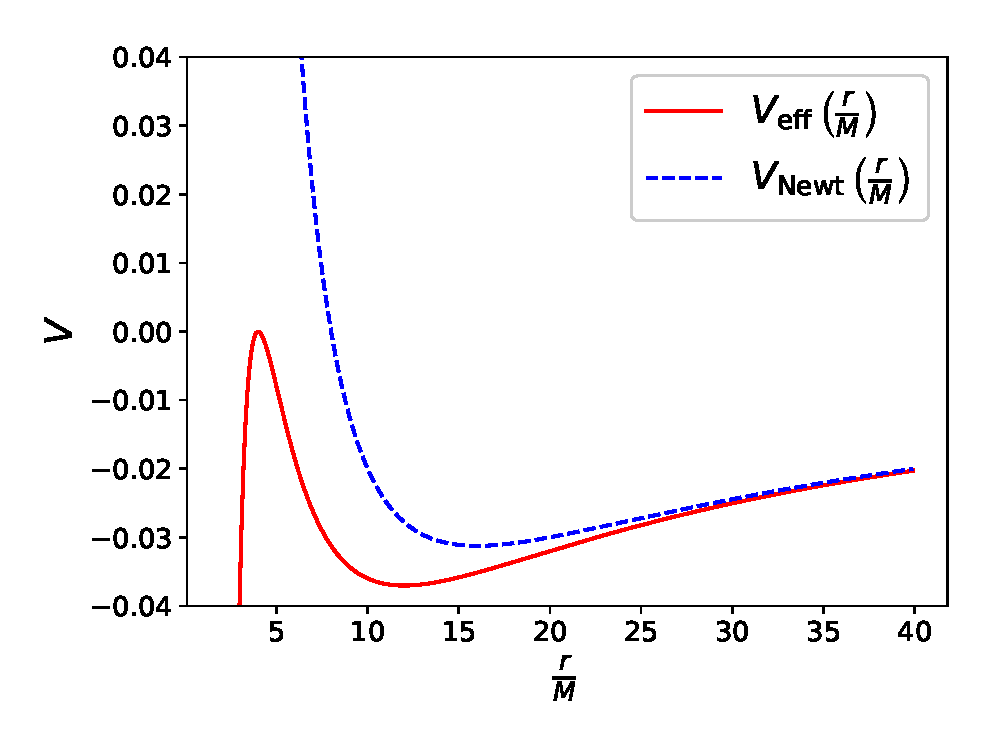
\includegraphics[width = \textwidth]{Figures/V_eff.eps}
    \caption{Effective potential defined in eq. \ref{cap1:eq:V_eff} against the
    Newtonian potential, $\frac{\ell}{M} = 4$. \\
    The $r^{-3}$ term dominates for $r \sim r_s$ and the
    particle can fall into the massive object.
    On the other hand the Newtonian potential presents its characteristic
    infinite centrifugal barrier.}
    \label{cap1:fig:V_effvsVN}
\end{minipage}
\hspace{0.009 \textwidth}
\begin{minipage}{0.49 \textwidth}
    \centering
    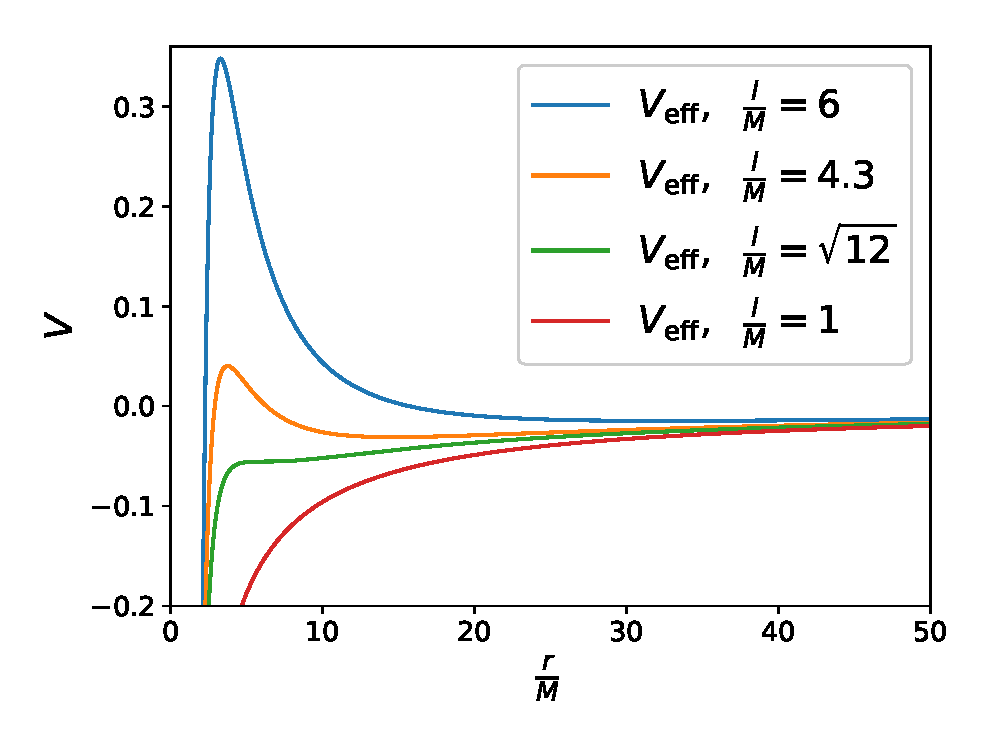
\includegraphics[width = \textwidth]{Figures/V_eff_tanti.eps}
    \caption{Plot of $V_{\rm eff}$ for
    $\frac{\ell}{M} = [1, \sqrt{12}, 4.3, 6]$.
    For $\frac{\ell}{M} = \sqrt{12}$ (green) there is only one stationary point
    and it is not stable.
    For $\frac{\ell}{M} = 1$ (red) there is no stationary point.
    The only stable points can be found for $\frac{\ell}{M} > \sqrt{12}$,
    in $r_{\rm min}$, defined in eq. \ref{cap1:eq:r_min_max}.}
    \label{cap1:fig:V_eff_tanti}
\end{minipage}
\end{figure}

Taking the derivative of $V_{\rm eff}$ with respect to $r$ gives us the
stationary points for $\frac{\ell}{M} \geq \sqrt{12}$.

\begin{subequations}
\begin{align}
    r_{+ / -} &= \frac{\ell^2}{2 M} \left[1 \pm
    \sqrt{1 - 12 \left( \frac{M}{\ell} \right)^2} \, \right]
    &&\frac{\ell}{M} > \sqrt{12} \label{cap1:eq:r_min_max} \\
    %
    r_{\rm ISCO} &= 6 M
    &&\frac{\ell}{M} = \sqrt{12} \label{cap1:eq:r_ISCO}
\end{align}
\label{cap1:eq:stationary_r}
\end{subequations}

In eq. \ref{cap1:eq:r_min_max} $r_-$ and $r_+$ correspond
to an unstable point and to a stable one respectively.

The case described by eq. \ref{cap1:eq:r_ISCO} represents the
\textit{innermost stable circular orbit} (ISCO).
As the name suggests, it is the smallest stable orbit that a particle can
theoretically follow.
It is shown in green in Figure \ref{cap1:fig:V_eff_tanti}.

For $\frac{\ell}{M} < \sqrt{12}$ there are no stationary points and the particle
is destined to fall towards the mass (red line in Figure
\ref{cap1:fig:V_eff_tanti}).

As in the Newtonian case a bound orbit exists only when $V_{\rm eff}$ has a
stable stationary point and the total energy given to the particle is not
greater than $V_{\rm eff}(r_-)$ (a more detailed explanation in
Section \ref{cap1:sec:stable_orbits}).

\newpage


\section{The Simplest Geodesics: Radial Infalls}

The simplest case we can consider is a radial infall where $\phi$ stays
constant.
From eq. \ref{cap1:eq:conserved_l} this implies $\ell = 0$.

Eq. \ref{cap1:eq:found_e} becomes


\begin{equation*}
    e^2 = \left(\dv{r}{\tau}\right)^2 + 1 - \frac{2M}{r}
\end{equation*}
\begin{equation}
    \dv{r}{\tau} = - \sqrt{e^2 - 1 + \frac{2 M}{r}} \, .
    \label{cap1:eq:radial_infall_ODE_1}
\end{equation}

Where we chose the negative root as the radius is decreasing.
Looking at the parameter $e$ in eq. \ref{cap1:eq:radial_infall_ODE_1} we can
distinguish 3 cases:

\begin{itemize}
    \item{$e^2 < 1$:} the particle has to start from a finite radius $r = R$
        for the argument of the square root to be positive;
    \item{$e = 1$:} the particle starts at rest from $r = \infty$ (that implies
        $\dv{t}{\tau} = 1$ at infinity so $e = 1$ from eq.
        \ref{cap1:eq:conserved_e});
    \item{$e^2 > 1$:} the particle starts from $r = \infty$, but with some
        inward velocity.
\end{itemize}

We choose to analyze the case where $e = 1$ so that eq.
\ref{cap1:eq:radial_infall_ODE_1} can be solved analytically.
We get

\begin{equation}
    \dv{r}{\tau} = - \sqrt{\frac{2 M}{r}} \, .
    \label{cap1:eq:radial_infall_ODE_2}
\end{equation}
\begin{equation*}
    r^{1/2} \mathrm{d}r = -(2M)^{1/2} \mathrm{d}\tau
\end{equation*}
\begin{equation}
    r(\tau) = \left(\frac{3}{2}\right)^{2/3}
    (2M)^{1/3} (\tau_* - \tau)^{2/3} \, .
    \label{cap1:eq:radial_infall_r_of_tau}
\end{equation}

Where $\tau_*$ is an integration constant that fixes the proper time $\tau$
when the particle arrives at $r = 0$.
An observer that falls together with the particle will measure a finite time
when he reaches $r = 2M$ and $\tau = \tau_*$ at $r = 0$.

On the contrary the experience from an observer far away from the source of
curvature, that measures the \Sh time $t$ it's much different.
To see this we can solve eq. \ref{cap1:eq:radial_infall_ODE_2} in respect to
the \Sh time $t$.
Using the chain rule to derive $r$ in respect of $t$ and eliminating the
dependence from $\tau$ using eq. \ref{cap1:eq:conserved_e} with $e = 1$, we get

\begin{align*}
    - \sqrt{\frac{2 M}{r}} = \dv{r}{\tau} = \dv{t}{\tau} \dv{r}{t}
    = \left(1 - \frac{2M}{r} \right)^{-1} \dv{r}{t}
\end{align*}
\begin{equation*}
    \dv{t}{r} = - \left(\frac{2 M}{r}\right)^{-1/2}
    \left(1 - \frac{2M}{r} \right)^{-1} \,  \, 
\end{equation*}

The integration is not as immediate as the previous one, but can be resolved
with simple techniques.
The result, fixing a similar time constant $t_*$ as before, is

\begin{equation}
    t = t_* + 2M \left[ -\frac{3}{2} \left(\frac{r}{2M}\right)^{3/2}
    - 2 \left(\frac{r}{2M}\right)^{1/2}
    + \ln \abs{\frac{(r/2M)^{1/2} + 1}{(r/2M)^{1/2} - 1}} \right] \, .
    \label{cap1:eq:radial_infall_r_of_t}
\end{equation}

We can't find $r(t)$ explicitly as was done previously, but the expression in
\ref{cap1:eq:radial_infall_r_of_t} already tells us that for
$r \rightarrow 2M$ the time measured by a far observer goes to infinity.
This implies that the distant observer will never see the particle reach
$r = 2M$ and enter the \Sh radius.
They will instead measure a signal infinitely redshifted as described by eq.
\ref{cap1:eq:redshift}, asymptotically going to $\omega_\infty = 0$.
That is why the \Sh radius is also referred to as a
\textit{source of infinite redshift}.
Figure \ref{cap1:fig:radial_infall} shows eq.
\ref{cap1:eq:radial_infall_r_of_tau} and eq
\ref{cap1:eq:radial_infall_r_of_t}, the integration constants $\tau_*$ and
$t_*$ where chosen to make both equations start from the same point
$r \simeq 12M$ at $\tau = t =  0$.

\begin{figure}[h]
    \centering
    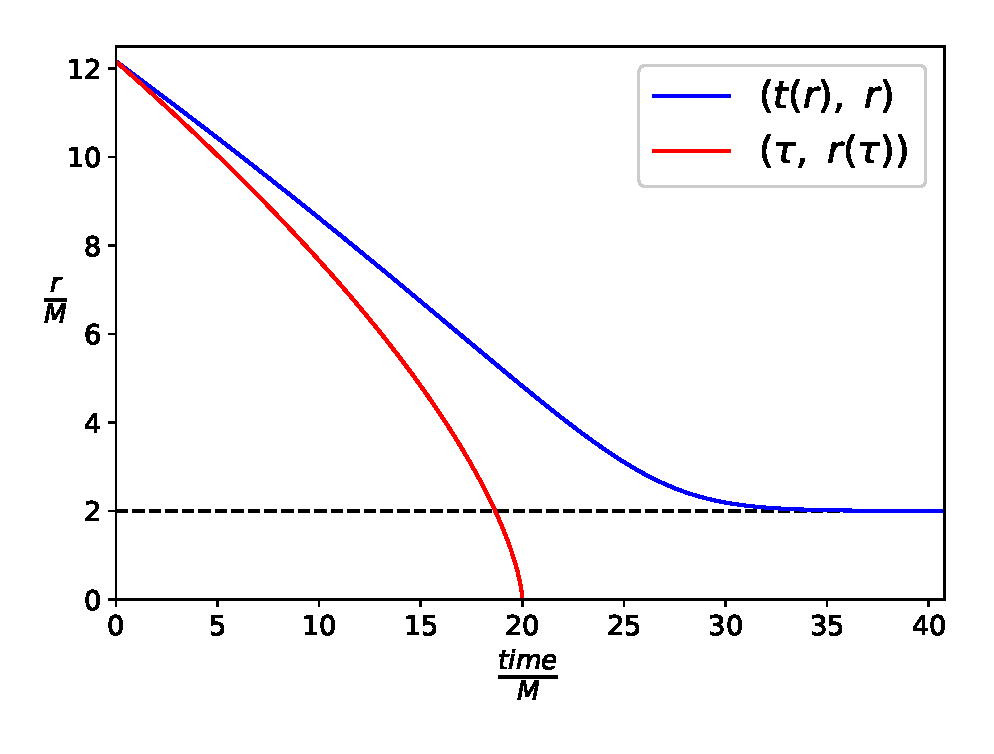
\includegraphics[width = 0.8 \textwidth]{Figures/radial_infall.eps}
    \caption{Eq. \ref{cap1:eq:radial_infall_r_of_tau} and eq.
    \ref{cap1:eq:radial_infall_r_of_t} describing the fall from
    $r \simeq 12M$ on.
    The integration constants $\tau_*$ and $t_*$ where fixed so that both
    equations started from the same $r(0)$.
    $r(\tau)$ gets to 0 quickly (at $\tau = \tau_*$), while $t(r)$ goes to
    infinity for $r \rightarrow r_s = 2M$. The \Sh radius $r_s$ is represented
    with the dashed black line.}
    \label{cap1:fig:radial_infall}

    % Va bene il grafico? credo potrebbe essere poco appropriato perché tempo 
    % proprio e tempo di \Sh dovrebbero essere uguali solo a r = \infty.
    % In teoria dovrei utilizzare l'equazione differenziale con e^2 < 1 in modo che
    % la particella parta da una distanza finita.
    % C'è il grafico fatto bene a pagina 344 del
    % Black Holes, White Dwarfs, and Neutron Stars (stuart L., Shapiro Saul A. Teukolsky)
    % che a sua volta è stato preso dal Gravitation Misner Thorne Wheeler 1973,
    % che ho trovato sull'Internet Archive
    % https://archive.org/details/GravitationMisnerThorneWheeler/page/n689/mode/2up
    % le 4 pagine sono in doc/
\end{figure}

\newpage


\section{Stable Orbits}
\label{cap1:sec:stable_orbits}

In Section \ref{cap1:sec:particle_orbits} we analyzed the role that
$\frac{\ell}{M}$ has on the effective potential $V_{\rm eff}$ defined in eq.
\ref{cap1:eq:V_eff} and found out that for $\frac{\ell}{M} > \sqrt{12}$ it has
two stationary points $r_{+ / -}$ defined in eq. \ref{cap1:eq:r_min_max}.

For clarity, we rewrite eq. \ref{cap1:eq:found_epsilon} below, accompanied by a
visual representation in Figure \ref{cap1:fig:V_eff_orbits}.

\begin{equation}
    \left( \dv{r}{\tau} \right)^2 = \mathcal E - V_{\rm eff} (r)
    \label{cap1:eq:like_newton}
\end{equation}

\begin{figure}[h]
    \centering
    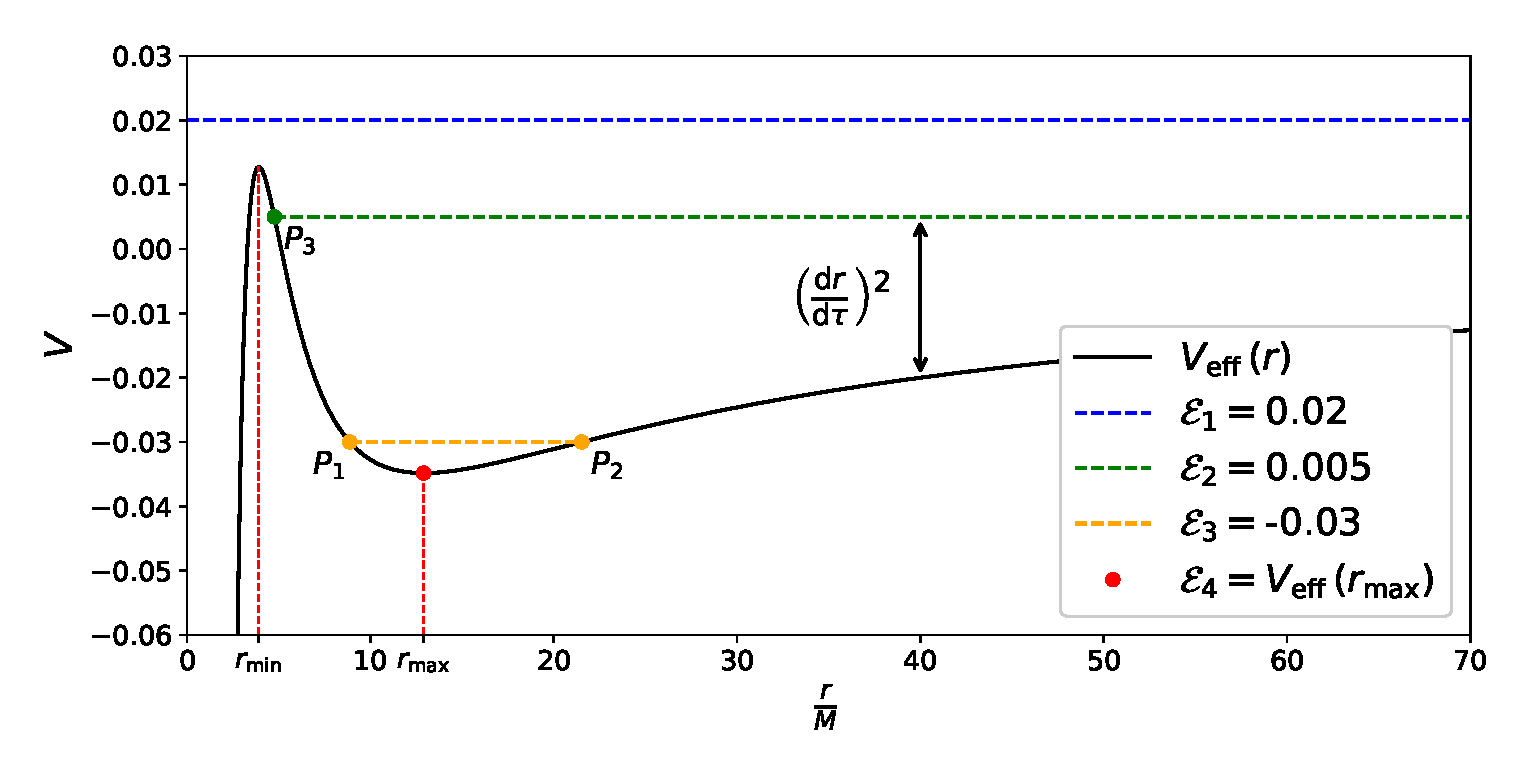
\includegraphics[width = \textwidth]{Figures/V_eff_orbits.eps}
    \caption{In black the effective potential with $\ell / M = 4.1$.
    The dashed lines, along with the red dot, represent possible values of
    $\mathcal E$ that give 4 different scenarios.
    Refer to the text for a detailed explanation. 
    \textit{This figure inspired from
    \cite[page 245, Figure 12.2]{shapiro2008black}.}}
    \label{cap1:fig:V_eff_orbits}
\end{figure}

From eq. \ref{cap1:eq:like_newton} we know that the particle can change its
distance $r$ from the massive object only if there is the energy
$\mathcal E - V_{\rm eff}$ to do so.
In Figure \ref{cap1:fig:V_eff_orbits}, $V_{\rm eff}$ with $\ell / M = 4.1$ is
represented along with 4 different values of $\mathcal E$.

The red full dot represents the case where the particle has exactly the energy
required to stay in the local minimum of the potential.
Here there is no \textit{spare} energy that the particle can use to move along
$r$.
This is the case of a circular orbit, and it will be explored in Section
\ref{cap1:ssec:circular_orbits}

In the yellow case, $\mathcal E = -0.03$, the particle has some \textit{spare}
energy (not enough to escape) to change its radius between the two turning
points $P_1$ and $P_2$
This results in an ellipse-like shape around the massive object.
\footnote{As we will see in Section \ref{cap1:sec:precession} it's not
exactly an ellipse as in the Newtonian case.}

Finally, the green case, $\mathcal E = 0.005$, and the blue one,
$\mathcal E = 0.02$, are not stable orbits.
In the first case, the particle has one turning point $P_3$ and has enough
energy to escape the potential well and go back towards infinity.
In the latter, the particle as a bigger energy than $V_{\rm eff} (r_-)$
and can fall into the massive object.


\subsection{Circular Orbits}
\label{cap1:ssec:circular_orbits}

As we have seen from Figure \ref{cap1:fig:V_eff_orbits} a particle can draw a
circular orbits if it has an energy $\mathcal E = V_{\rm eff}(r_+)$.
It is possible to find the relationship between the energy $e$
and angular momentum $\ell$ that makes this possible.

First of all, the four-velocity of the particle will be

\begin{equation}
    u^\mu = \left(\dv{t}{\tau}, 0, 0, \dv{\phi}{\tau} \right)
    = \left(\dv{t}{\tau}, 0, 0, \dv{t}{\tau} \Omega \right)
    = u^t (1, 0, 0, \Omega) \,
    \label{cap1:eq:circular_orbit_u}
\end{equation}

Where we defined $\Omega := \dv{\phi}{t}$: the rate of which $\phi$ changes with
respect to the \Sh time $t$.
Using eq. \ref{cap1:eq:conserved_e} and eq. \ref{cap1:eq:conserved_l}, $\Omega$
can be rewritten as

\begin{equation}
    \Omega = \dv{\phi}{t} = \dv{\tau}{t} \dv{\phi}{\tau} =
    \frac{1}{r^2} \left(1 - \frac{2M}{r} \right) \frac{\ell}{e}\, .
    \label{cap1:eq:Omega}
\end{equation}

A second equation for $\frac{\ell}{e}$ comes with the restriction that the
particle must orbit at the minimum of $V_{\rm eff}$, from eq.
\ref{cap1:eq:r_min_max}

\begin{equation}
    r = \frac{\ell^2}{2 M} \left[1 +
    \sqrt{1 - 12 \left( \frac{M}{\ell} \right)^2} \, \right] \, .
    \label{cap1:eq:r_min}
\end{equation}

Using eq. \ref{cap1:eq:found_e} the derivative of $r$ vanishes
and we can write everything as

\begin{equation}
    e^2 = \left(1 + \frac{\ell^2}{r^2} \right)
    \left(1 - \frac{2M}{r}\right) \, .
    \label{cap1:eq:circular_orbit1}
\end{equation}

Instead of substituting $r$ from eq. \ref{cap1:eq:r_min} into eq.
\ref{cap1:eq:circular_orbit1}, it is easier to solve eq. \ref{cap1:eq:r_min} for
$1 / \ell^2$ obtaining

\begin{equation}
    \frac{1}{\ell^2} = \frac{1}{M r} - \frac{3}{r^2} \, ,
\end{equation}

and then use it to rewrite eq. \ref{cap1:eq:circular_orbit1} as

\begin{align*}
    \frac{e^2}{\ell^2} &= \left(\frac{1}{\ell^2} + \frac{1}{r^2} \right)
    \left(1 - \frac{2M}{r}\right)
    %
    = \left(\frac{1}{M r}
    - \frac{3}{r^2}
    + \frac{1}{r^2}\right)
    \left(1 - \frac{2M}{r}\right) 
    %
    = \frac{1}{M r} \left(1
    - \frac{2 M}{r} \right)^2 \\
\end{align*}
\begin{equation}
    \frac{\ell}{e} = \sqrt{M r} \left(1
    - \frac{2 M}{r} \right)^{-1}
    \label{cap1:eq:circular_orbit2}
\end{equation}

We can finally substitute eq. \ref{cap1:eq:circular_orbit2} into eq.
\ref{cap1:eq:Omega} to get

\begin{equation}
    \Omega^2 = \frac{M}{r^3}
    \label{cap1:eq:Omega2}
\end{equation}

that gives the angular velocity observed from infinity of a particle in a
circular orbit.
With the value of $\Omega$ found in eq. \ref{cap1:eq:Omega2} we can find the
normalization of the four-velocity defined in \ref{cap1:eq:circular_orbit_u}.

\begin{align*}
    - 1 = \mathbf{u \cdot u} = g_{\nu \mu} u^\nu u^\mu
    &= (u^t)^2 \left[- \left(1 - \frac{2M}{r}\right) + r^2 \Omega^2 \right] \\
    (u^t)^2 &= \left[ 1 - \frac{2M}{r} - \frac{M}{r}\right]^{-1} \\
    u^t &= \left( 1 - \frac{3M}{r} \right)^{-1/2} \\
\end{align*}

Therefore, we have

\begin{equation}
    u^\mu = \left( 1 - \frac{3M}{r} \right)^{-1/2}
    \left( 1, 0, 0, \sqrt{\frac{M}{r^3}} \right)
\end{equation}


\subsection{General Shapes and Precession}
\label{cap1:sec:precession}

To complete the discussion on bound orbit we can have a look at a more general
case, where $V_{\rm eff} < \mathcal E < 0$.
If we want to characterize the shape of the orbit, as always restricted to the
$xy$ plane, we need to express $\phi$ as a function of $r$.
To do so we can use eq. \ref{cap1:eq:conserved_l} and eq. \ref{cap1:eq:found_e}
and rewrite them respectively as

\begin{subequations}
\begin{align}
    \dv{\phi}{\tau} &= \frac{\ell}{r^2} \label{cap1:eq:shape1} \\
    \dv{r}{\tau} &= \pm \sqrt{e^2 - \left(1 + \frac{\ell^2}{r^2}\right)
    \left(1 - \frac{2M}{r}\right)} \label{cap1:eq:shape2} \, .
\end{align}
\label{cap1:eq:to_find_shape}
\end{subequations}

This time we had no reason to keep one sign or the other in eq.
\ref{cap1:eq:shape2}.
Dividing \ref{cap1:eq:shape2} into \ref{cap1:eq:shape1} gives

\begin{equation}
    \dv{\phi}{r} = \pm \frac{\ell}{r^2}
    \left[e^2 - \left(1 + \frac{\ell^2}{r^2}\right)
    \left(1 - \frac{2M}{r}\right)\right]^{-1/2}
    \label{cap1:eq:shape}
\end{equation}

The function $\phi(r)$ can be found simply by integrating the right-hand side.
The result can be expressed in terms of elliptic functions but not in a very
enlightening way for those not familiar with them
\footcite[page 202]{hartle2021gravity}.

An interesting parameter to study is the \textit{precession}, defined as

\begin{equation}
    \delta \phi_{\rm prec} = \Delta \phi - 2 \pi
    \label{cap1:eq:precession}
\end{equation}

To define $\Delta \phi$ consider the turning points $P_1$ and $P_2$ in Figure
\ref{cap1:fig:V_eff_orbits}.
\textit{One orbit} is complete when the particle starts from the inner turning
point, $P_1$, and gets back to it.
We can equivalently consider $P_2$ as a starting and ending point.
$\Delta \phi$ is the angle swept during one orbit.
It's also useful to notice that the angle swept in one orbit is twice the angle
swept between $P_1$ and $P_2$, thus we can rewrite $\Delta \phi$ as

\begin{figure}[h]
    \centering
    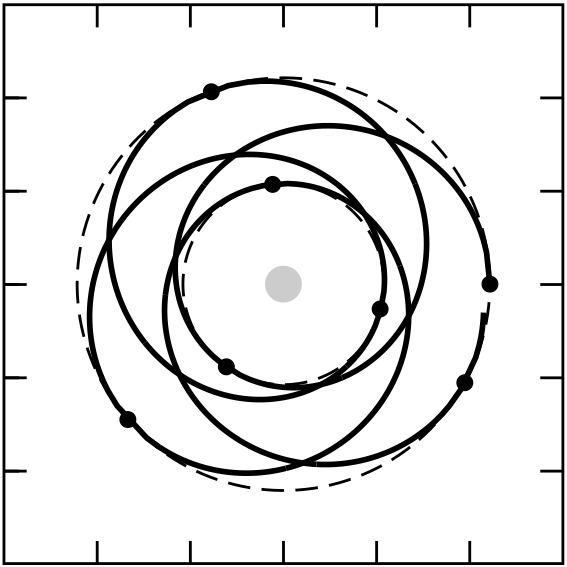
\includegraphics[width = 0.5 \textwidth]{Figures/precession_bozza.png}
    \caption{placeholder}
    \label{cap1:fig:precession}
\end{figure}

\begin{equation}
    \Delta \phi = \int_{P_1}^{P_2} \dv{\phi}{r} \mathrm{d}r
    = 2 \ell \int_{r_1}^{r_2} \frac{1}{r^2}
    \left[e^2 - \left(1 + \frac{\ell^2}{r^2}\right)
    \left(1 - \frac{2M}{r}\right)\right]^{-1/2} \mathrm{d}r
    \label{cap1:eq:delta_phi}
\end{equation}

By the definition of the turning points, $r_1$ and $r_2$, the integral we need
to compute is between the two zeros of the denominator contained in square
brackets.
To check the correspondence with the Newtonian case we can solve the integral
in \ref{cap1:eq:delta_phi} neglecting the $r^{-3}$ term and remembering the
definition of $\mathcal E$ from eq. \ref{cap1:eq:found_epsilon}:

\begin{equation*}
    \Delta \phi = 2 \ell \int_{r_1}^{r_2} \frac{1}{r^2} \left[\mathcal E -
    \frac{\ell^2}{r^2}\ + \frac{2M}{r} \right]^{-1/2} \mathrm{d}r
\end{equation*}

Making the substitution $u = 1 / r$ and using the root of the denominator as
the bounds of integration we get

\begin{equation}
    \Delta \phi
    = 2 \int_{u_2}^{u_1} \frac{\mathrm{d} u}{\sqrt{(u_1 - u)(u - u_2)}} 
    = 2 \pi \quad \quad \forall u_1 \neq u_2
\end{equation}

where $u_{1/2} = \frac{1}{r_{1/2}}$, but the integral is $\pi$ for every $u_1$
and $u_2$.

% Problem 15 to get the expression inthe first order of 1 / c^2 ?

\newpage


\section{Light Ray orbits}

When working with light, more properly photons, we define the four-velocity
using the \textit{affine parameter} $\lambda$.

\begin{equation*}
    u^\mu = \dv{x^\mu}{\lambda} \, .
\end{equation*}

The conserved quantities $e$ and $\ell$ defined in \ref{cap1:eq:conserved_e} and
\ref{cap1:eq:conserved_l} are the same, with the only difference of using
$\lambda$ instead of the proper time $\tau$.

\begin{subequations}
    \begin{align*}
        e &= \left( 1 - \frac{2M}{r} \right) \dv{t}{\lambda} \\
        \ell &= r^2 \sin^2 \theta \dv{\phi}{\lambda} \, .
    \end{align*}
\end{subequations}

We can therefore restrict the motion of the light ray motion to the $xy$ plane
as we did with massive particle and write four-velocity as

\begin{equation*}
    u^\mu
    = \left(\dv{t}{\lambda}, \dv{r}{\lambda}, 0, \frac{\ell}{r^2} \right) \, .
\end{equation*}

The only difference lies, as described in eq.
\ref{cap1:eq:u_normalization_light}, in the normalization of $\mathbf u$, that
is $\mathbf{u \cdot u} = 0$.

So, with the same intent we had when we found eq. \ref{cap1:eq:found_e} we can
write

\begin{equation*}
    0 = g_{\nu \mu} u^\nu u^\mu =
    - \left(1 - \frac{2M}{r} \right) \left(\dv{t}{\lambda} \right)^2
    + \left(1 - \frac{2M}{r} \right)^{- 1} \left(\dv{r}{\lambda} \right)^2
    + \frac{\ell^2}{r^2}
\end{equation*}

and then rearrange

\begin{equation}
    \frac{1}{b^2} = \frac{1}{\ell^2} \left( \dv{r}{\lambda} \right)^2
    + W_{\rm eff} (r) \, .
    \label{cap1:eq:found_b}
\end{equation}

Where we defined another effective potential, one that acts on light rays only,
as

\begin{equation}
    W_{\rm eff} (r) = \frac{1}{r^2} \left( 1 - \frac{2M}{r} \right)
    \label{cap1:eq:W}
\end{equation}

and a different constant for the energy

\begin{equation}
    b^2 = \frac{\ell^2}{e^2} \, .
    \label{cap1:eq:b}
\end{equation}

